\graphicspath{{./ninth/img}} % path to graphics

\section{Изменение текущей модели}
Откроем предыдущую модель и удалим из нее некоторые параметры и графики.
Добавим два параметра timeMean, коэффициент и переменную время выполнения.
timeMean по умолчанию зададим как 29 типа int, коэффициент зададим как 1 типа double, время выполнения зададим как double.

\begin{image}
	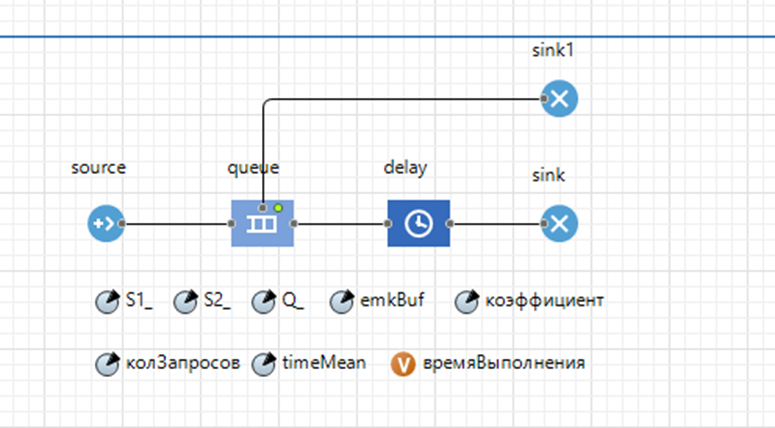
\includegraphics[width=1\textwidth]{img1}
	\caption{Добавление новых параметров}
	\label{fig:model}
\end{image}

Также выделим объект sink и в поле Действие при входе установим следующий код:
if( sink.in.count() == количествоЗапросов ){ времяВыполнения = time(); stopSimulation();}

\clearpage

\section{Создание нового эксперимента}
Создадим новый эксперимент типа варьирования параметров.
В свойствах укажем максимальный размер памяти – 256мб, а количество прогонов – 9604.
Также добавим параметры и зададим их значение. В разделе Действия Java установим код data.reset();

\begin{image}
	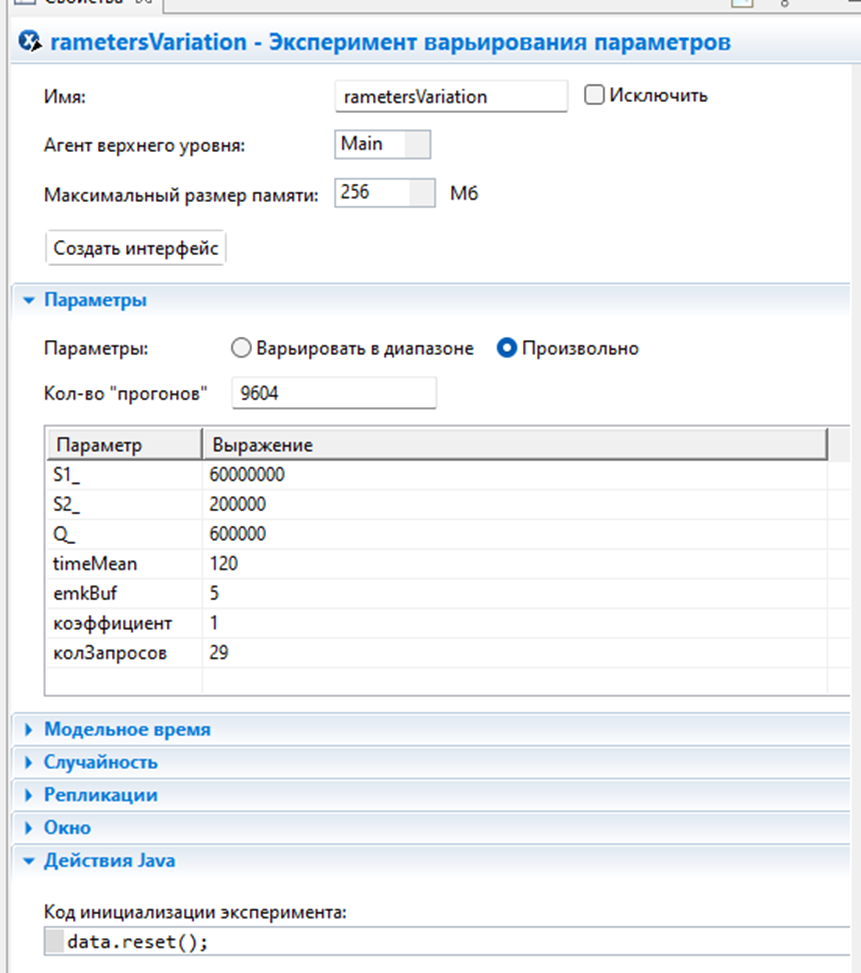
\includegraphics[width=1\textwidth]{img2}
	\caption{Создание эксперимента}
	\label{fig:data}
\end{image}

\clearpage

\section{Создание интерфейса}
Создадим интерфейс, на котором будет изображена гистограмма, ее данные и данные с ее средним значением.

\begin{image}
	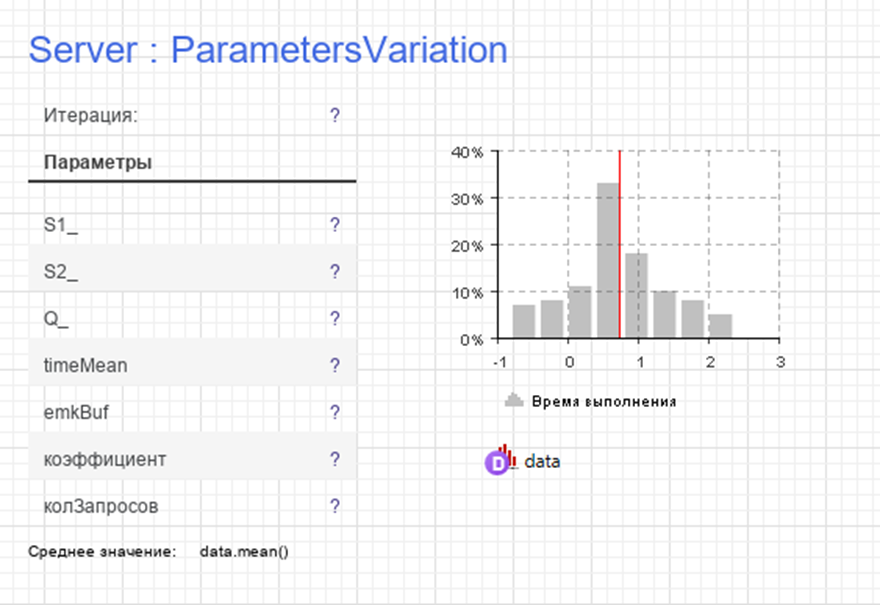
\includegraphics[width=1\textwidth]{img3}
	\caption{Создание эксперимента}
	\label{fig:interface}
\end{image}

\clearpage

\section*{Вывод}
В ходе выполнения данной практической работы была выполнена обратная задача путем создания модели сервера.

